\documentclass{article}
\usepackage{graphicx}
\usepackage[hyphens]{url}

\author{Ian Leinbach and Corin Rose}
\title{Inter-Planetary ID}

\begin{document}

\maketitle

\begin{center}
\textbf{Abstract} 
\end{center}

A universally agreed upon format for defining what data constitutes an ID would allow for interoperability between services. If this format is based on IPLD and represented as hash-linked data, we can leverage IPFS to store and share this information in a distributed way and let users maintain control of their data.\footnote{\url{https://ipld.io/}}\footnote{\url{https://ipfs.io/}} By building off of amazing work done in distributed systems, we can create this format as a way of standardizing how a human exists on the Internet, in much the same way that, for example, Unicode standardized the way we represent arbitrarily complex symbols with data.  

\section{Introduction}
In IPID, an ID is simply a a folder of data hosted on IPFS which contains your data footprint--that is, all of the data you want to be associated with your public Internet identity, from contact info to published writing. We share this data by assigning an IPNS link to this data, which you can then give to people out of band (e.g. on a buisness card, or via a text). Then, you can update the IPFS folder pointed to by this name whenever you update your data, and anyone can always access this data with that same IPNS name. 

\section{Format}

\subsection{Data Serialization}

In an IPID folder, data should be future proof and self-describing in the sense of Multiformats.\footnote{\url{https://multiformats.io/}} Multiformats let us encode data in a consistent way, prefacing it with metadata about its content, and includes both a human-readable and binary representation. For example we can reference \texttt{foo.jpg}, a file stored on our own local machine over http on port 8000, by \texttt{/ip4/127.0.0.1/tcp/8000/http\-/foo.jpg}. This human-readable format can translated into a binary format with a lookup table for values of each protocol. Many types of content already do something like this, for example by declaring \texttt{<!DOCTYPE html>} in an HTML document. Any file in an IPID folder should make clear the way it is storing data.   

\subsection{Profile}

\begin{figure}[h]
  \centering
  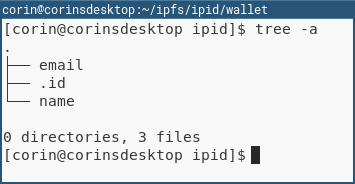
\includegraphics[width=.5\textwidth]{resources/basic_profile.png}
  \caption{A minimal profile.}
\end{figure}

We see in figure 1 an example of the most basic profile you can have. It consists of a "name," an "email," and a ".id" file. The name and email are both just plain text files with the name and email respectively. In this context, the names of the files act as sufficient metadata to describe the content. The name does not have to be a real name, it can be psuedononymous. The .id file contains a version field and the IPNS name of the given profile. It acts as a flag that this folder is in fact an IPID folder. An ID needs to have at minimum a name and some kind of contact information, like email or phone, in addition to the .id file. \par
Profiles can also include payment information in a "wallet" folder. For example, if you wish to post a Bitcoin recieving address to your profile, you can create "wallet/btc," a text file that contains your BTC address. See figure 2. We can similarly extend this model to include any kind of data.

\begin{figure}[h]
  \centering
  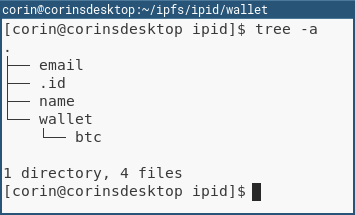
\includegraphics[width=.5\textwidth]{resources/basic_profile_wallet.png}
  \caption{A profile with a Bitcoin recieving address.}
\end{figure}

\subsection{Extensions}

We can easily define extensions to this format. A simple example is the wallet folder we saw above. Similarly, we could create a "blog" folder which contains a bunch of text files, each of which is a new blog post. Then, anyone could write code that found this profile, looked through all of these posts, and formatted them nicely as a blog. One could easily use this as a decentralized content management system for their own websites, or someone could offer a service that read blog data from a given profile over IPFS and formatted it into a profile resembling modern social media websites. \par
Organizations could also define their own extension paths to any depth. For example, if Vassar College wanted to integrate their data about me into my profile, they could create a "vassar" folder to add to the root folder, which would then include for example a student\_id file, and a transcript file, and so on. This third party format could also include subfolders. \\
Going further, a social media site or game could create a folder within one's data footprint to store data, leaving the user in control of their data. When someone wants to add to or change your content, they must go through you first. We enable secure content management through IPFS.

\subsection{IPFS}

The Inter-Planetary Filesystem is a new Web. It addresses two of the flaws of HTTP: the World Wide Web uses location-based addressing, and operates within a client-server model. These two factors have been a centralizing force on the Web, enabling big corporations like Facebok, Google, Microsoft, and Apple to dominate the industry. These corporations offer identity services more complete than IPID, but they depend on centralized security models, where trusted institutions take responsibility for our data. We see time and time again that this model for security does not work in the decentralized world of the Internet. Attacks on a network can come from anywhere, and if there is a central point of failure it is bound to be targeted. IPFS takes inspiration from decentralized technologies like Git, BitTorrent, and Blockchains to address these problems with the Web. With IPFS, we now use content-based addressing, so we can look for a file and download it BitTorrent style from everyone who has. This also builds in data integrity checks. IPFS uses a Distributed Hash Table to build a global routing table, storing which node stores what data. With this technology, we can take IPFS to be the new Web, and describe IPID as a standard sitting above IPFS.

\subsection{Hosting on IPFS}

We can easily host our IPID folder on IPFS.

\begin{figure}[h]
  \centering
  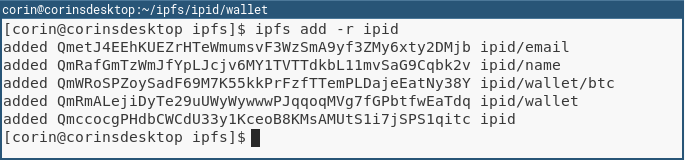
\includegraphics[width=.9\textwidth]{resources/profile_to_ipfs.png}
  \caption{Adding your IPID folder to IPFS.}
\end{figure}

Once we add this folder with our IPID data to IPFS, as seen in figure 3, it can be accessed from anywhere at \\
  \texttt{/ipfs/QmccocgPHdbCWCdU33y1KceoB8KMsAMUtS1i7jSPS1qitc} \\ 
For example, to find the Bitcoin address, we can look for \\
  \texttt{/ipfs/QmccocgPHdbCWCdU33y1KceoB8KMsAMUtS1i7jSPS1qitc/wallet/btc} 
and read what we know will be the hash of a Elliptic Curve public key.  
This is not ideal, however, because now you must send a new IPFS link every time you update this information. Luckly, IPFS let's use name content! 

\subsection{IPNS}

IPNS provides us a PKI global namespace for addressing, and a way to resolve these addresses over IPFS. We can thus generate an IPNS name by hashing a public key. IPFS typically uses RSA. This functionality is conveniently built into the reference implementation of IPFS. 

\begin{figure}[h]
  \hspace*{-2cm}
  \centering
  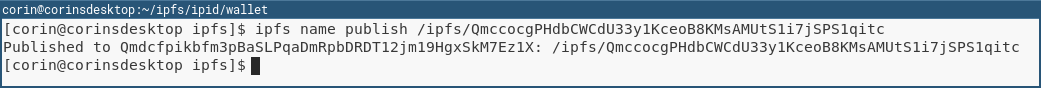
\includegraphics[width=.75\paperwidth]{resources/publish_profile.png}
  \caption{Publishing your IPID folder to your IPNS name.}
\end{figure}

Now, you can share \texttt{/ipns/Qmdcfpikbfm3pBaSLPqaDmRpbDRDT12jm19HgxSkM7Ez1X} with anyone and they will be able to find your up to date data over IPFS!

\section{Security}
 
This technology will act as a layer above IPFS. Thus, the first question we must ask is what security guarentees does IPFS give us. The structure of IPFS, a merkle DAG, is inherently invulnreable to data manipulation--that is, it guarentees data integrity, so if I give you a IPFS link in the form of a content hash, you know that the data you receive is what I intended to send. IPNS is built to be interoperable and run on many different asymmetric cryptography schemes, but uses industry standard RSA by default. This is of course depend on the hardness of factoring primes, which Quantum Computers will be able to break with Shor's algorithm once we figure out that whole decoherence thing, at which point IPFS will have no issue transitioning to a new key system--although this would require users to update their IPNS names. Although our format does not include specifications for encrypted data, one could easily encrypt data themselves and put it on IPFS, only sharing the keys with those they would like, or adopt whatever scheme they wish. Encryption will eventually be built into IPFS at the protocol layer, making this even easier. 

\section{Use Cases}

\subsection{Business Card}

One way to use this data footprint is to share it on a business card. This card can include a small QR code that encodes the IPNS path to the folder with your data. You can give out this business card to as many people as you'd like, and they will always be able to view your most up to date public data. 

\begin{figure}[h]
  \centering
  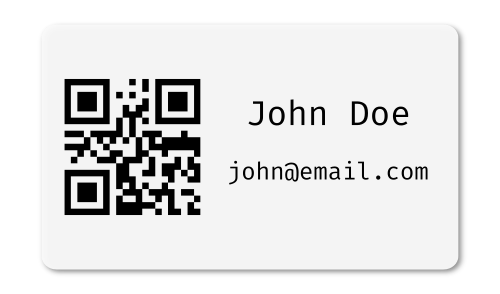
\includegraphics{resources/business_card.png}
  \caption{An example of a business card with a QR code that links to an ID over IPNS.}
\end{figure}

\subsection{Reference Implementation}

We will develop a reference implementation of this format which aims to be a Minimum Viable Product (MVP), demonstrating the core functionality of IPID without investigating creative uses of the protocol. With this in mind, the reference implementation will aim to work like a traditional blogging website. It will allow users to create and manage their IPID, and look at a nicely formatted version of other users IPIDs. 

\subsubsection{Client-Side IPFS Node}

We will utilize the js-IPFS in-browser IPFS node to let the user interact with IPFS themselves, from our website. This API can interact with a node running on the computer, or with the IPFS Companion, a cross-platform browser extension that runs a Javascript IPFS node in your browser.\footnote{\url{https://github.com/ipfs-shipyard/ipfs-companion}} We will encourage average users to opt for the browser extension. The home page will detect whether the user is running an IPFS node on their computer with this API. If they are and the node's name links to a folder with a .id file, the site will detect this and automatically "log-in" the user--that is, display a view profile button rather than a create profile button, options to edit your profile from our site, and so on. If there is a node running but no ID on it, the site will allow the user to create a profile 

\subsubsection{SQLite Database}

The site will include a SQLite database which stores data about users who create an ID through the site. We will also "mirror" all of the users ID data on our own IPFS node. Users can then search on our site for other users with any data. If it is an IPNS name, the site can check if it is in the database, and if not make a request over IPFS for the files. If users are in our database, however, the search features are much more extensive, and they can search by anything that would be in the profile. 

\subsubsection{Blog Extension}

This web site would utilize the blog extension mentioned above. This is simply a folder within one's IPID named blog, which contains some files. These files can be any kind of markup format, as long as they are self describing. For example, one can use simply name their blog posts with an extension marking its type. There is no need to make all of the files the same type, as seen in figure 6. 

\begin{figure}[h]
  \centering
  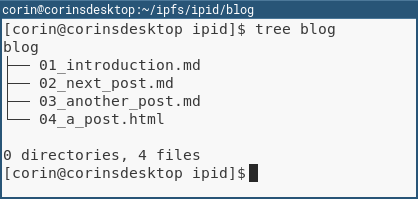
\includegraphics[width=.75\linewidth]{resources/blog_example.png}
  \caption{An example of a blog with a few posts.}
\end{figure}

\section{Conclusion}

\end{document}
